%!TEX root = ../out/07-branch-SL.tex

\begin{document}

\title[Branching]
{Branching algorithms}

\begin{frame}
  \titlepage
\end{frame}

\lecturenotes{\maketitle}

\begin{frame}
 \slides{\frametitle{Outline}}
 \tableofcontents
\end{frame}

\section{Branching algorithms}

\begin{frame}
 \slides{\frametitle{Branching Algorithm}}

 \begin{block}{Branching Algorithm}
  \begin{itemize}
   \item \alert{Selection}: Select a local configuration of the problem instance
 %\pause
   \item \alert{Recursion}: Recursively solve subinstances
 %\pause
   \item \alert{Combination}: Compute a solution of the instance based on the solutions of the subinstances
  \end{itemize}
 \end{block}
 
 %\pause
 \begin{itemize}
  \item \alert{Halting} rule: $0$ recursive calls
  \item \alert{Simplification} rule: $1$ recursive call
  \item \alert{Branching} rule: $\ge 2$ recursive calls
 \end{itemize}

\end{frame}

\begin{frame}
 \frametitle{Example: Our first \VC\ algorithm}

\begin{algorithm}[H]
\SetArgSty{}

\alert{Algorithm $\text{vc1}(G,k)$}\;
\BlankLine

   \lnl{algvctl:1}\If(\tcp*[f]{all edges are covered}){$E = \emptyset$} {
      \lnl{algvctl:2}\Return{Yes}
   }
   \lnl{algvctl:3}\ElseIf(\tcp*[f]{we cannot select any vertex}){$k \le 0$} {
      \lnl{algvctl:4}\Return{No}
   }
   \lnl{algvctl:5}\Else {
      \lnl{algvctl:6}Select an edge $uv\in E$\;
      \lnl{algvctl:7} \Return{$\text{vc1}(G - u, k-1) \;\vee\; \text{vc1}(G - v, k-1)$}
   }
\end{algorithm}

\end{frame}

\section{Running time analysis}

\begin{frame}
 \frametitle{Search trees}
 
 \textbf{Recall}: A \alert{search tree} models the recursive calls of an algorithm.\\
 For a $b$-way branching where the parameter $k$ decreases by $a$ at each recursive call, the number of nodes is at most $b^{k/a}\cdot (k/a+1)$.
 
 \begin{center}
 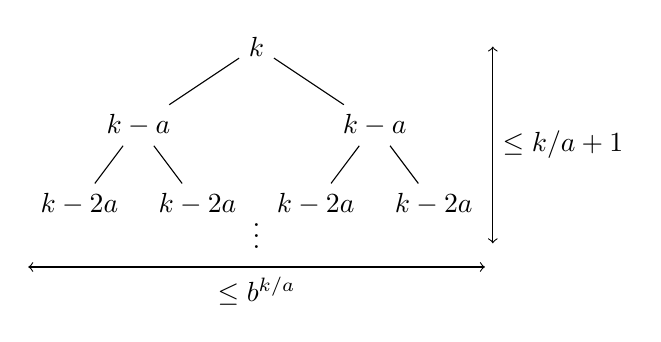
\begin{tikzpicture}
  [level distance=10mm,
   level 1/.style={sibling distance=30mm},
   level 2/.style={sibling distance=15mm}]
 \node {$k$}
  child {node {$k-a$}
   child {node {$k-2a$}}
   child {node {$k-2a$}}
  }
  child {node {$k-a$}
   child {node {$k-2a$}}
   child {node {$k-2a$}}
  };
  \node at (0,-2.3) {$\vdots$};
  \draw[<->] (3,0)--(3,-2.5) node[midway,right] {$\le k/a+1$};
  \draw[<->] (-2.9,-2.8)--(2.9,-2.8) node[midway,below] {$\le b^{k/a}$};
 \end{tikzpicture}
 \end{center}
 
 If $k/a$ and $b$ are upper bounded by a function of $k$,
 and the time spent at each node is \FPT\ (typically, polynomial),
 then we get an \FPT\ running time.

\end{frame}


\section{Feedback Vertex Set}

\begin{frame}
	\slides{\frametitle{Feedback Vertex Set}}

 \noindent
 A \alert{feedback vertex set} of a multigraph $G=(V,E)$ is a set of vertices $S\subseteq V$ such that $G-S$ is acyclic.
 
 \pbDef{\textsc{Feedback Vertex Set}}{Multigraph $G=(V,E)$, integer $k$}{$k$}{Does $G$ have a feedback vertex set of size at most $k$?}

 \begin{center}
	\begin{tikzpicture}[scale=0.7]
	\node[vertex]  (a) at (1.5,3  ) {};
	\node[vertex] (b) at (3  ,3  ) {};
	\node[vertex] (c) at (0  ,1.5) {};
	\node[selected]                 (d) at (1.5,1.5) {};
	\node[selected]                 (e) at (3  ,1.5) {};
	\node[vertex] (f) at (1.5,0  ) {};
	\node[vertex]                 (g) at (3  ,0  ) {};
	\node[vertex] (h) at (4.5,0  ) {};
	\node[vertex] (i) at (0,3) {};
	\draw[line width=1.5pt]     (i) -- (a) -- (b) -- (e) -- (h) -- (g) -- (f) -- (d) -- (g) -- (e) -- (a) -- (c) -- (d);
	\draw[line width=1.5pt] (a) .. controls +(-0.3,-0.5) and +(-0.3,0.5) .. (d);
	\draw[line width=1.5pt] (a) .. controls +( 0.3,-0.5) and +( 0.3,0.5) .. (d);
	\draw[line width=1.5pt] (e) .. controls +( 0.2,1) and +(1,0) .. (e);
	\end{tikzpicture}
 \end{center}

\end{frame}

\begin{frame}{Simplification Rules}

 We apply the first \alert{applicable}\footnote[frame]{A rule is \alert{applicable} if it modifies the instance.}
simplification/halting rule.
 
 \begin{block}{(Finished)}
  If $G$ is acyclic and $k\ge 0$, then return \Yes.
 \end{block}
 \begin{block}{(Budget-exceeded)}
  If $k< 0$, then return \No.
 \end{block}

 \pause
 \begin{block}{(Loop)}
  If $G$ has a loop $vv\in E$, then set $G \leftarrow G-v$ and $k\leftarrow k-1$.
 \end{block}
 
 \pause
 \begin{block}{(Multiedge)}
  If $E$ contains an edge $uv$ more than twice, remove all but two copies of $uv$.
 \end{block}

\end{frame}

\begin{frame}
 \slides{\frametitle{Simplification Rules II}}

 \begin{block}{(Degree-1)}
  If $\exists v\in V$ with $d_G(v)\le 1$, then set $G \leftarrow G-v$.
 \end{block}
	
\end{frame}

\begin{frame}
 \slides{\frametitle{Simplification Rules III}}

 \begin{block}{(Degree-2)}
  If $\exists v\in V$ with $d_G(v)=2$, then denote $vu,vw$ its two incident edges and set $G \leftarrow G'=(V\setminus \{v\},(E\setminus \{vu,vw\}) \cup \{uw\})$.
 \end{block}

 \pause
 \begin{lemma}
  (Degree-2) is sound.
 \end{lemma}
 \begin{proof}\slides{\small}
  Suppose $S$ is a feedback vertex set of $G$ of size at most $k$.
  Let
  \begin{align*}
   S' &=
    \begin{cases}
     S & \text{if } v\notin S\\
     (S \setminus \{v\}) \cup \{u\} & \text{if } v\in S.
    \end{cases}
  \end{align*}
  Now, $|S'|\le k$ and $S'$ is a feedback vertex set of $G'$ since every cycle in $G'$ corresponds to a cycle in $G$, with, possibly, the edge $uw$ replaced by the walk $(u,v,w)$.
  
  \smallskip
  Suppose $S'$ is a feedback vertex set of $G'$ of size at most $k$.
  Then, $S'$ is also a feedback vertex set of $G$.
 \end{proof}
 
\end{frame}

\begin{frame}{Remaining issues}

 \begin{itemize}
  \item A select--discard branching decreases $k$ in only one branch
  \item One could branch on all the vertices of a cycle, but the length of a shortest cycle might not be bounded by any function of $k$
 \end{itemize}
 
 \pause
 Idea:
 \begin{itemize}
  \item An acyclic graph has average degree $<2$
  \item After applying simplification rules, $G$ has average degree $\ge 3$
  \item The selected feeback vertex set needs to be incident to many edges
  \item Does a feedback vertex set of size at most $k$ contain at least one vertex among the $f(k)$ vertices of highest degree?
 \end{itemize}

\end{frame}

\begin{frame}{The fvs needs to be incident to many edges}
 
 \begin{lemma}
  If $S$ is a feedback vertex set of $G=(V,E)$, then
  \begin{align*}
   \sum_{v\in S} (d_G(v)-1) \ge |E|-|V|+1
  \end{align*}
 \end{lemma}
 \pause
 \begin{proof}
  Since $F=G-S$ is acyclic, $|E(F)| \le |V|-|S|-1$.\\
  Since every edge in $E \setminus E(F)$ is incident with a vertex of $S$, we have
  \begin{align*}
   |E| &= |E| - |E(F)| + |E(F)|\\
       &\le \left(\sum_{v\in S} d_G(v)\right) +(|V|-|S|-1)\\
       &= \left(\sum_{v\in S} (d_G(v)-1)\right) +|V|-1.
  \end{align*}
 \end{proof}

\end{frame}

\begin{frame}{The fvs needs to contain a high-degree vertex}
 \begin{lemma}
  Let $G$ be a graph with minimum degree at least 3 and let $H$ denote a set of $3k$ vertices of highest degree in $G$.\\
  Every feedback vertex set of $G$ of size at most $k$ contains at least one vertex of $H$.
 \end{lemma}
 \pause
 \begin{proof}\slides{\small}
  Suppose not. Let $S$ be a feedback vertex set with $|S|\le k$ and $S\cap H = \emptyset$.
  Then,
  \begin{align*}
   2|E|-|V| &= \sum_{v\in V} (d_G(v)-1)\\
            &= \sum_{v\in H} (d_G(v)-1) + \sum_{v\in V\setminus H} (d_G(v)-1)\\
            &\ge 3\cdot ( \sum_{v\in S} (d_G(v)-1) ) + \sum_{v\in S} (d_G(v)-1)\\
            &\ge 4\cdot ( |E|-|V|+1)\\
  \Leftrightarrow \quad 3|V| &\ge 2|E|+4.
  \end{align*}
  But this contradicts the fact that every vertex of $G$ has degree at least $3$.
 \end{proof}

\end{frame}


\begin{frame}{Algorithm for Feedback Vertex Set}
 
 \begin{theorem}
  \textsc{Feedback Vertex Set} can be solved in $O^*((3k)^k)$ time.
 \end{theorem}
 \begin{proof}[Proof (sketch).]
  \begin{itemize}
   \item Exhaustively apply the simplification rules.
   \item The branching rule computes $H$ of size $3k$, and branches into subproblems $(G-v,k-1)$ for each $v\in H$.
  \end{itemize}

 \end{proof}
 
 \lecturenotes{
 Current best:\\ $O^*(3.460^k)$ deterministic \cite{IwataK19},\\ $O^*(2.7^k)$ time randomized \cite{LiN19}
 }


\end{frame}

\section{Maximum Leaf Spanning Tree}

\begin{frame}
	\slides{\frametitle{Maximum Leaf Spanning Tree}}
 
 A \alert{leaf} of a tree is a vertex with degree 1.
 A \alert{spanning tree} in a graph $G=(V,E)$ is a subgraph of $G$ that is a tree and has $|V|$ vertices.\\
 
 \pbDef{\textsc{Maximum Leaf Spanning Tree}}{connected graph $G$, integer $k$}{$k$}{Does $G$ have a spanning tree with at least $k$ leaves?}
\end{frame}


\begin{frame}
	\frametitle{Property}
	
	A \alert{$k$-leaf tree} in $G$ is a subgraph of $G$ that is a tree with at least $k$ leaves.\\
	A \alert{$k$-leaf spanning tree} in $G$ is a spanning tree in $G$ with at least $k$ leaves.
	\begin{lemma}
		Let $G=(V,E)$ be a connected graph.\\
		$G$ has a $k$-leaf tree $\Leftrightarrow$ $G$ has a $k$-leaf spanning tree.
	\end{lemma}
	\begin{proof}
	 $(\Leftarrow)$: trivial
	 
	 $(\Rightarrow)$: Let $T$ be a $k$-leaf tree in $G$. By induction on $x := |V|-|V(T)|$, we will show that $T$ can be extended to a $k$-leaf spanning tree in $G$.\newline
	 Base case: $x=0$ \checkmark.\newline
	 Induction: $x>0$, and assume the claim is true for all $x'<x$. Choose $uv\in E$ such that $u\in V(T)$ and $v\notin V(T)$. Since $T' := (V(T)\cup\{v\},E(T)\cup\{uv\})$ has $\ge k$ leaves and $<x$ external vertices, it can be extended to a $k$-leaf spanning tree in $G$ by the induction hypothesis.
	\end{proof}
\end{frame}

\begin{frame}{Strategy}

 \begin{itemize}
  \item The branching algorithm will check whether $G$ has a $k$-leaf tree.
  \item A tree with $\ge 3$ vertices has at least one \alert{internal} (= non-leaf) vertex.
  \item ``Guess'' an internal vertex $r$, i.e., do a $|V|$-way branching fixing an initial internal vertex $r$.
  \pause
  \item In any branch, the algorithm has computed
   \begin{itemize}
    \item $T$ -- a tree in $G$
    \item $I$ -- the internal vertices of $T$, with $r\in I$
    \item $B$ -- a subset of the leaves of $T$ where $T$ may be extended: the boundary set
    \item $L$ -- the remaining leaves of $T$
    \item $X$ -- the external vertices $V\setminus V(T)$
   \end{itemize}
  \pause
  \item The question is whether $T$ can be extended to a $k$-leaf tree where all the vertices in $L$ are leaves.
 \end{itemize}
 
\end{frame}


\begin{frame}{Simplification Rules}

 Apply the first applicable simplification rule:
 
 \begin{block}{(Halt-Yes)}
  If $|L|+|B|\ge k$, then return \Yes.
 \end{block}

 \begin{block}{(Halt-No)}
  If $|B|=0$, then return \No.
 \end{block}
 
 \begin{block}{(Non-extendable)}
  If $\exists v\in B$ with $N_G(v) \cap X = \emptyset$, then move $v$ to $L$. 
 \end{block}

\end{frame}


\begin{frame}{Branching Lemma}

 \begin{lemma}[Branching Lemma]
  Suppose $u\in B$ and there exists a $k$-leaf tree $T'$ extending $T$ where $u$ is an internal vertex.\\
  Then, there exists a $k$-leaf tree $T''$ extending $(V(T) \cup N_G(u), E(T) \cup \{uv : v \in N_G(u) \cap X\})$.
 \end{lemma}
 \pause
 \begin{proof}
  Start from $T'' \leftarrow T'$ and perform the following operation for each $v\in N_G(u)\cap X$.
  
  If $v \notin V(T')$, then add he vertex $v$ and the edge $uv$.\\
  Otherwise, add the edge $uv$, creating a cycle $C$ in $T$ and remove the other edge of $C$ incident to $v$. This does not decrease the number of leaves, since it only increases the number of edges incident to $u$, and $u$ was already internal.
 \end{proof}

\end{frame}


\begin{frame}{Follow Path Lemma}

 \begin{lemma}[Follow Path Lemma]
  Suppose $u\in B$ and $|N_G(u) \cap X|=1$. Let $N_G(u) \cap X = \{v\}$.\\
  If there exists a $k$-leaf tree extending $T$ where $u$ is internal, but no $k$-leaf tree extending $T$ where $u$ is a leaf, then there exists a $k$-leaf tree extending $T$ where both $u$ and $v$ are internal.
 \end{lemma}
 \pause
 \begin{proof}
  Suppose not, and let $T'$ be a $k$-leaf tree extending $T$ where $u$ is internal and $v$ is a leaf. But then, $T-v$ is a $k$-leaf tree as well.
 \end{proof}

\end{frame}


\begin{frame}{Algorithm}

 \begin{itemize}
  \item Apply halting \& simplification rules
  \item Select $u\in B$. Branch into
  \begin{itemize}
   \item $u\in L$
   \item $u\in I$. In this case, add $X\cap N_G(u)$ to $B$ (Branching Lemma). 
   \begin{itemize}
    \item In the special case where $|X\cap N_G(u)|=1$, denote $\{v\}=X\cap N_G(u)$, make $v$ internal, and add $N_G(v)\cap X$ to $B$, continuing the same way until reaching a vertex with at least 2 neighbors in $X$ (Follow Path Lemma).
    \item In the special case where $|X\cap N_G(u)|=0$, return \No.
   \end{itemize}
  \end{itemize}
  \medskip
  \pause
  \item In one branch, a vertex moves from $B$ to $L$; in the other branch, $|B|$ increases by at least 1.
 \end{itemize}
\end{frame}


\begin{frame}{Running time analysis}
 
 \begin{itemize}
  \item Consider the ``measure'' $\mu := 2k - 2|L| - |B|$
  \item We have that $0 \le \mu \le 2k$
  \item Branch where $u\in L$:
   \begin{itemize}
    \item $|B|$ decreases by $1$, $|L|$ increases by 1
    \item $\mu$ decreases by 1
   \end{itemize}
  \item Branch where $u\in I$.
   \begin{itemize}
     \item $u$ moves from $B$ to $I$
     \item $\ge 2$ vertices move from $X$ to $B$
     \item $\mu$ decreases by at least 1
   \end{itemize}
 \end{itemize}
 \medskip
 \begin{itemize}
  \item Binary search tree of height $\le \mu \le 2k$
 \end{itemize}
\end{frame}

\begin{frame}
 \frametitle{Result for Maximum Leaf Spanning Tree}
 \begin{theorem}[\cite{KneisLR11}]
  \textsc{Maximum Leaf Spanning Tree} can be solved in $O^*(4^k)$ time.
 \end{theorem}
 
 \lecturenotes{
 Current best: $O(3.188^k)$ \cite{Zehavi18}
 }
\end{frame}


\section{Further Reading}

\begin{frame}
 \slides{\frametitle{Further Reading}}

  \begin{itemize}
   \item Chapter 3, \emph{Bounded Search Trees} in \cite{CyganFKL+15}
%   Marek Cygan, Fedor V.\ Fomin, \L ukasz Kowalik, Daniel Lokshtanov, D{\'a}niel Marx, Marcin Pilipczuk, Micha\l Pilipczuk, and Saket Saurabh. Parameterized Algorithms. Springer, 2015.
   \item Chapter 3, \emph{Bounded Search Trees} in \cite{DowneyF13}
%         Rodney G. Downey and Michael R. Fellows. Fundamentals of Parameterized Complexity. Springer, 2013.
   \item Chapter 8, \emph{Depth-Bounded Search Trees} in \cite{Niedermeier06}
%         Rolf Niedermeier. Invitation to Fixed Parameter Algorithms. Oxford University Press, 2006.
  \end{itemize}

\end{frame}

\begin{frame}[t, allowframebreaks]
	\slides{\frametitle{References}}
	\printbibliography
\end{frame}


\end{document}
